\documentclass[runningheads]{llncs}

\usepackage{amssymb}
\setcounter{tocdepth}{3}
\usepackage{multirow}
\usepackage{graphicx,amsmath, amsfonts, color, cite, subfig, stfloats, url}% times
\usepackage{lscape}
\usepackage{epsfig}
\usepackage{rotating}

\usepackage{url}
\urldef{\mailsa}\path|jceberio001@ikasle.ehu.es,|
\urldef{\mailsb}\path|{alexander.mendiburu,ja.lozano}@ehu.es|
\newcommand{\keywords}[1]{\par\addvspace\baselineskip
\noindent\keywordname\enspace\ignorespaces#1}

\usepackage{array}

\newcolumntype{x}[1]{%
>{\centering\hspace{0pt}}p{#1}}%

\begin{document}

\mainmatter  % start of an individual contribution

% first the title is needed
\title{Introducing the Mallows Model on\\ Estimation of Distribution Algorithms}

% a short form should be given in case it is too long for the running head
\titlerunning{Introducing the Mallows Model on Estimation of Distribution Algorithms}

% the name(s) of the author(s) follow(s) next
%
% NB: Chinese authors should write their first names(s) in front of
% their surnames. This ensures that the names appear correctly in
% the running heads and the author index.
%
\author{Josu Ceberio%
%\thanks{Please note that the LNCS Editorial assumes that all authors have used
%the western naming convention, with given names preceding surnames. This determines
%the structure of the names in the running heads and the author index.}%
\and Alexander Mendiburu\and Jose A. Lozano}
%
\authorrunning{Josu Ceberio, Alexander Mendiburu, Jose A. Lozano}
% (feature abused for this document to repeat the title also on left hand pages)

% the affiliations are given next; don't give your e-mail address
% unless you accept that it will be published
\institute{Intelligent Systems Group\\
Faculty of Computer Science\\
The University of The Basque Country\\
Manuel de Lardizabal pasealekua, 1\\
20018 Donostia - San Sebastian, Spain\\
\mailsa\\
\mailsb\\
\url{http://www.sc.ehu.es/isg}}

%
% NB: a more complex sample for affiliations and the mapping to the
% corresponding authors can be found in the file "llncs.dem"
% (search for the string "\mainmatter" where a contribution starts).
% "llncs.dem" accompanies the document class "llncs.cls".
%

\toctitle{Introducing the Mallows Model on Estimation of Distribution Algorithms}
\tocauthor{Authors' Instructions}
\maketitle

\begin{abstract}
Estimation of Distribution Algorithms are a set of algorithms that belong to the field of Evolutionary Computation. 
Characterized by the use of probabilistic models to learn the (in)dependencies between the variables of the optimization problem, these algorithms have been applied to a wide set of academic and real-world optimization problems, achieving competitive results in most scenarios. However, they have not been extensively developed for permutation-based problems. In this paper we introduce a new EDA approach specifically designed to deal with permutation-based problems. In this paper, our proposal estimates a probability distribution over permutations by means of a distance-based exponential model called the Mallows model. In order to analyze the performance of the Mallows model in EDAs, we carry out some experiments over the Permutation Flowshop Scheduling Problem (PFSP), and compare the results with those obtained by two state-of-the-art EDAs for permutation-based problems.
\keywords{Estimation of Distribution Algorithms, Probabilistic Models, Mallows Model, Permutations, Flow Shop Scheduling Problem} 
\end{abstract}

\section{Introduction}

Estimation of Distribution Algorithms (EDAs)~\cite{muhlenbein96,larra01a,pelikan00a} are a set of Evolutionary Algorithms (EAs). However, unlike other EAs, at each step of the evolution, EDAs learn a probabilistic model from a population of solutions trying to explicitly express the interrelations between the variables of the problem. The new offspring is then obtained by sampling the probabilistic model. The algorithm stops when a certain criterion is met, such as a maximum number of generations, homogeneous population, or lack of improvement in the last generations.          

Many different approaches have been given in the literature to deal with permutation problems by means of EDAs. However, most of these proposals are adaptations of classical EDAs designed to solve discrete or continuous domain problems. Discrete domain EDAs follow the path-representation codification~\cite{Robles02} to encode permutation problems. These approaches learn, departing from a dataset of permutations, a probability distribution over a set $\Omega=\{0,\ldots,n-1\}^n,\hspace{0.3cm} \hbox{where} \hspace{0.3cm} n\in\mathbb{N}$. Therefore, the sampling of these models has to be modified in order to provide permutation individuals. Algorithms such as Univariate Marginal Distribution Algorithm (UMDA), Estimation of Bayesian Networks Algorithm (EBNAs), or Mutual Information Maximization for Input Clustering (MIMIC) have been applied with this encoding to different problems~\cite{DBLP:journals/pr/BengoetxeaLBPB02,Robles02,mendiburu}.

Adaptations of continuous EDAs~\cite{Bosman01, Robles02,mendiburu} use the Random Keys representation~\cite{DBLP:journals/informs/Bean94} to encode a solution with random numbers. These numbers are used as sort keys to obtain the permutation. Thus, to encode a permutation of length $n$, each index in the permutation is assigned a value (key) from some real domain, which is usually taken to be the interval [0, 1]. Subsequently, the indexes are sorted using the keys to get the permutation. The main advantage of random keys is that they always provide feasible solutions, since each encoding represents a permutation. However, solutions are not processed in the permutation space, but in the largely redundant real-valued space. For example, for length $3$ permutation, strings (0.2, 0.1, 0.7) and (0.4, 0.3, 0.5) represent the same permutation (2, 1, 3).

The limitations of these direct approaches, both in the discrete and continuous domains, encouraged the research community of EDAs to implement specific algorithms for solving permutation-based problems. Bosman and Thierens introduced the ICE~\cite{Bosman01,DBLP:conf/ppsn/BosmanT02} algorithm to overcome the bad performance of Random Keys in permutation optimization. The ICE replaces the sampling step with a special crossover operator which is guided by the probabilistic model, guaranteeing feasible solutions.

In~\cite{DBLP:journals/ijar/RomeroL09} a new framework for EDAs called Recursive EDAs (REDAs) is introduced. REDAs is an optimization strategy that consists of separately optimizing different subsets of variables of the individual.

Tsutsui et al.~\cite{DBLP:conf/ppsn/Tsutsui02,Tsutsui06nodehistogram} propose two new models to deal with permutation problems. The first approach is called Edge Histogram Based Sampling Algorithm (EHBSA). EHBSA builds an Edge Histogram Matrix (EHM), which models the edge distribution of the indexes in the selected individuals. A second approach called Node Histogram Based Sampling Algorithm (NHBSA), introduced later by the authors, models the frequency of the indexes at each absolute position in the selected individuals. Both algorithms simulate new individuals by sampling the marginals matrix. In addition, the authors proposed the use of a template-based method to create new solutions. This method consists of randomly choosing an individual from the previous generation, dividing it into $c$ random segments and sampling the indexes for one of the segments, leaving the remaining indexes unchanged.
A generalization of these approaches was given by Ceberio et al.~\cite{ceberio11a}, where the proposed algorithm learns $k$-order marginal models.

As stated in~\cite{ceberio11b}, Tsutsui's EHBSA and NHBSA approaches yield the best results for several permutation-based problems, such as Traveling Salesman Problem, Flow Shop Scheduling Problem, Quadratic Assignment Problem or Linear Ordering Problem. However, these approaches are still far from achieving optimal solutions, which means that there is still room for improvement. Note that the introduced approaches do not estimate a probability distribution over the space of permutations that allow us to calculate the probability of a given solution in a closed form. Motivated by this issue and working in that direction, we present a new EDA which models an explicit probability distribution over the permutation space: the Mallows EDA.

The remainder of the paper is as follows: Section 2 introduces the optimization problem we tackle: The Permutation Flow Shop Scheduling Problem. In Section 3 the Mallows model is introduced. In section 4, some preliminary experiments are run to study the behavior of the Mallows EDA. Finally, conclusions are drawn in Section 5.

\section{The Permutation Flowshop Scheduling Problem}

The Flowshop Scheduling Problem~\cite{flowshop06} consists of scheduling $n$ jobs $(i=1,\ldots,n)$ with known processing time on $m$ machines $(j=1,\ldots,m)$. A job consists of $m$ operations and the $j$-th operation of each job must be processed on machine $j$ for a specific time. A job can start on the $j$-th machine when its $(j-1)$-th operation has finished on machine $(j-1)$, and machine $j$ is free. If the jobs are processed in the same order on different machines, the problem is named as Permutation Flowshop Scheduling Problem (PFSP). The objective of the PFSP is to find a permutation that achieves a specific criterion such as minimizing the total flow time, the makespan, etc.
The solutions (permutations) are denoted as $\sigma=(\sigma_1,\sigma_2,\ldots,\sigma_n)$ where $\sigma_i$ represents the job to be processed in the $i$-th position. For instance, in a problem of 4 jobs and 3 machines, the solution $(2,3,1,4)$, indicates that job $2$ is processed first, next job 3 and so on.

Let $p_{i,j}$ denote the processing time for job $i$ on machine $j$, and $c_{i,j}$ denote the completion time of job $i$ on machine $j$. Then, $c_{\sigma_i,j}$ is the completion time of the job scheduled in the $i$-th position on machine $j$. $c_{\sigma_i,j}$ is computed as $c_{\sigma_i,j}=p_{\sigma_i,j} + max\{c_{\sigma_i,j-1},c_{\sigma_{i-1},j} \}$. As this paper addresses the makespan performance measure, the objective function $F$  is defined as follows: \[F(\sigma_1,\sigma_2,\ldots,\sigma_n)=c_{\sigma_{n},m}\]

As can be seen, the solution of the problem is given by the processing time of the last job $\sigma_n$ in the permutation, since this is the last job to finish.

\section{The Mallows Model}

The Mallows model \cite{mallows} is a distance-based exponential probability model over permutation spaces. Given a distance $d$ over permutations, it can be defined by two parameters: the central permutation $\sigma_0$, and the spread parameter $\theta$. (\ref{equation1}) shows the explicit form of the probability distribution over the space of permutations:

\begin{equation}
P(\sigma)= \frac{1}{\psi(\theta)}e^{-\theta d (\sigma, \sigma_0)}
\label{equation1}
\end{equation}
%
where $\psi(\theta)$ is a normalization constant. When $\theta>0$, the central permutation $\sigma_0$ is the one with the highest probability value and the probability of the other $n!-1$ permutations exponentially decreases with the distance to the central permutation (and the spread parameter $\theta$). Because of these properties, the Mallows distribution is considered analogous to the Gaussian distribution on the space of permutations (see Fig.~\ref{F:MallowsPD}). Note that when $\theta$ increases, the curve of the probability distribution becomes more peaked at $\sigma_0$.
\vspace{-0.5cm}
\begin{figure}
\centering
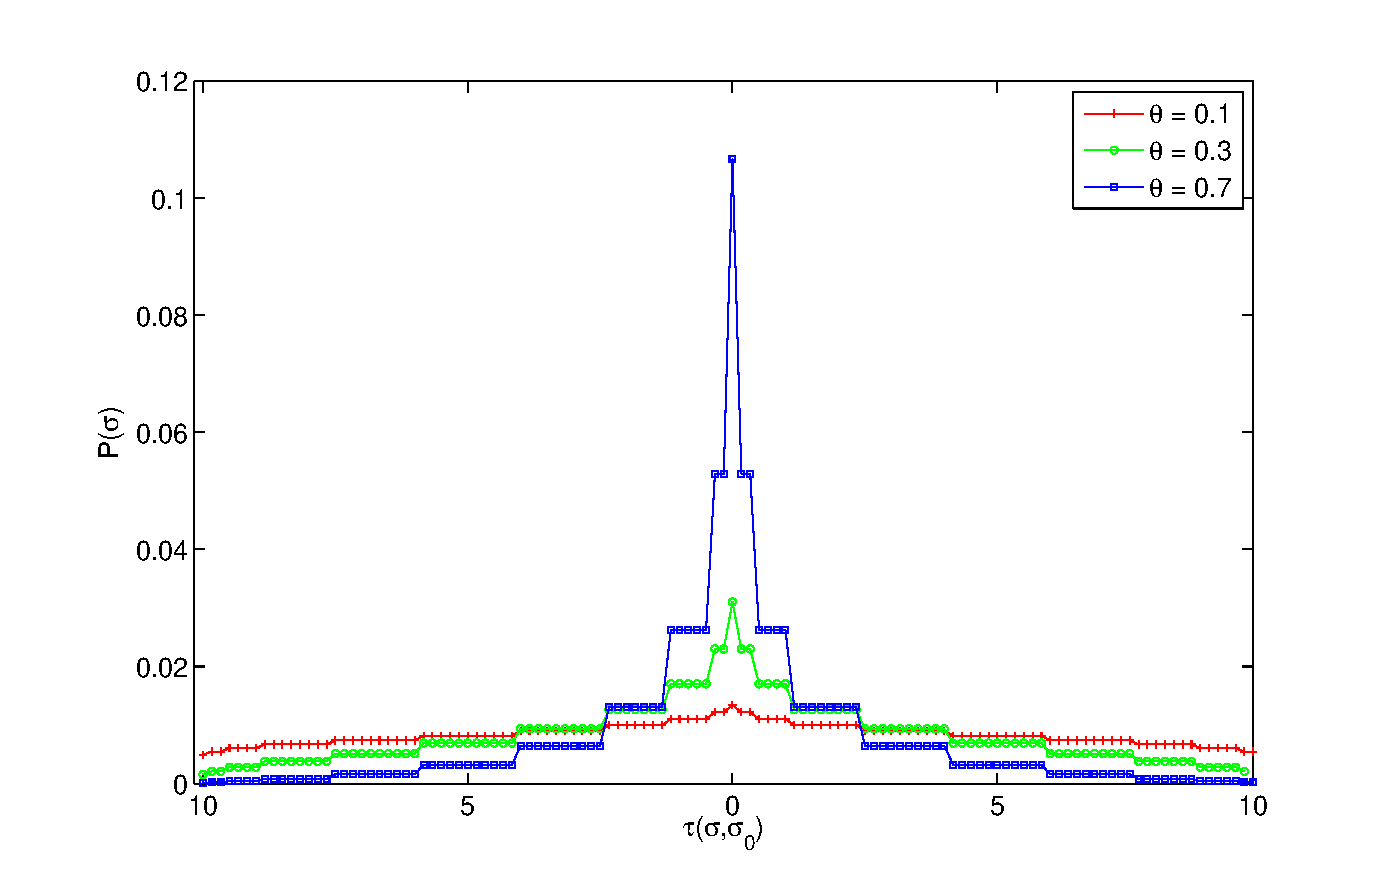
\epsfig{file=images/MallowsPD_6,height=7cm}
\caption{Mallows probability distribution with the Kendall-$\tau$ distance for different spread parameters. In this case, the dimension of the problem is $n=5$.}
\label{F:MallowsPD}
\end{figure}
\vspace{-0.5cm}

\subsection{Kendall-$\tau$ Distance}
The Mallows model is not tied to a specific distance. In fact, it has been used with different distances in the literature such as Kendall, Cayley or Spearman~\cite{gmallows}. For the application of the Mallows model in EDAs, we have chosen the Kendall-$\tau$ distance. This is the most commonly used distance with the Mallows model, and in addition, its definition resembles the structure of a basic neighborhood system in the space of permutations. Given two permutations $\sigma_1$ and $\sigma_2$, the Kendall-$\tau$ distance counts the total number of pairwise disagreements between both of them i.e., the minimum number of adjacent swaps to convert $\sigma_1$ into $\sigma_2$. 
Formally, it can be written as 

\begin{align*}
\tau(\sigma_1, \sigma_2)=|\{(i,j) : i<j,\, & (\sigma_1(i) < \sigma_1(j) \land \sigma_2(i)>\sigma_2(j) ) \\ 
 \lor \,& (\sigma_2(i) < \sigma_2(j) \land \sigma_1(i)>\sigma_1(j) )  \, \}|.
\end{align*}

The above metric can be  equivalently written as 

\begin{equation}
\tau (\sigma_1, \sigma_2)=\sum_{j=1}^{n-1}V_j(\sigma_1, \sigma_2)
\end{equation}

\noindent
where $V_j(\sigma_1, \sigma_2)$ is the minimum number of adjacent swaps  to set in the $j$-th position of $\sigma_1$, $\sigma_1(j)$, the value $\sigma_2(j)$. This decomposition allows to factorize the distribution as a product of independent univariate exponential models\cite{meila2007-conrank}, one for each $V_j$ and that (see (\ref{E:factorization1}) and (\ref{E:factorization2})).

\begin{equation}
\psi(\theta) = \prod_{j=1}^{n-1}\psi_j(\theta) = \frac{1-e^{-(n-j+1)\theta}}{1-e^{-\theta}}
\label{E:factorization1}
\end{equation}

\begin{equation}
P(\sigma)= \frac{e^{-\theta \sum_{j=1}^{n-1}V_j(\sigma,\sigma_0)}}{\prod_{j=1}^{n-1}\psi_j(\theta)} = \prod_{j=1}^{n-1}\frac{e^{-\theta V_j(\sigma,\sigma_0)}}{\psi_j(\theta)}
\label{E:factorization2}
\end{equation}

This property of the model is essential to carry out an efficient sampling. Furthermore, one can uniquely determine any $\sigma$ by the $n-1$ integers $V_1(\sigma)$, $V_2(\sigma)$,\ldots,$V_{n-1}(\sigma)$ defined as 
\begin{equation}
V_j(\sigma,I)=\sum_{l>j}1_{[l\prec_{\sigma}j]}
\end{equation}

\noindent
where $I$ denotes the identity permutation (1, 2,\ldots$n$) and $l\prec_{\sigma}j$ means that $l$ precedes $j$ (i.e. is preferred to $j$) in permutation $\sigma$.

\subsection{Learning and Sampling a Mallows Model}

At each step of the EDA, we need to learn a Mallows model from the set of selected individuals (permutations). Therefore, given a dataset of permutations $\{\sigma_0,\sigma_1,\ldots,\sigma_N\}$ we need to estimate $\sigma_0$ and $\theta$. In order to do that, we use the maximum likelihood estimation method. The log-likelihood function can be written as 
\begin{equation} 
log \,\,l ( \sigma_1, ..., \sigma_N | \sigma_0,\theta)= - N \sum_{j=1}^{n-1}(\theta \bar{V}_j + \text{log}\, \psi_j (\theta))
\end{equation}
\noindent
where $\bar{V}_j= \sum_{i=1}^{N}V_j(\sigma_i, \sigma_0)/N$, i.e. $\bar{V}_j$ denotes the observed mean for $V_j$. 

The problem of finding the central permutation or consensus ranking is called rank aggregation and it is, in fact, equivalent to finding the MLE estimator of $\sigma_0$, which is NP-hard. One can find several methods for solving this problem, both exact \cite{cohen10} and heuristic \cite{meilaTractable}.
In this paper we propose the following: first, the average of the values at each position is calculated, and then, we assign index $1$ to the position with the lowest average value, next index 2 to the second lowest position, and so on until all the $n$ values are assigned.

Once $\sigma_0$ is known, the estimation of $\theta$ maximizing the log-likelihood  is immediate by numerically solving the following equation:

\begin{equation}
	\sum_{j=1}^{n-1}\bar{V}_j= \frac{n-1}{e^{\theta}-1}-\sum_{j=1}^{n-1}\frac{n-j+1}{e^{(n-j+1)\theta}-1}
	\label{E:thetas}
\end{equation}
%
In general, this solution has no closed form expression, but can be solved numerically by standard iterative algorithms such as Netwon-Rapshon.

In order to sample, we consider a bijection between the $V_j$-s and the permutations. By sampling the probability distribution of the $V_j$-s defined by (\ref{E:samplingEq}), a $V_j$-s vector is obtained. The new permutations are calculated applying the sampled $V_j$ vector to the consensus permutation $\sigma_0$ following a specific algorithm~\cite{meila2007-conrank}. 

\begin{equation}P[V_j(\sigma\sigma_0^{-1},I)=r]=\frac{e^{-\theta r}}{\psi_j(\theta)}\label{E:samplingEq}\end{equation}

\section{Experiments}

Once the Mallows model has been introduced, we devote this section to carrying out some experiments in order to analyze the behavior of this new EDA. As stated previously, the variance of the Mallows model is controlled by a spread parameter $\theta$, and therefore it will be necessary to observe how the model behaves according to different values of $\theta$. In a second phase, and based on the values previously obtained, the Mallows EDA will be run for some instances of the FSP problem. In addition, for comparison purposes, two state-of-the-art EDAs~\cite{ceberio11b} will be also included, in particular Tsutsui's EHBSA and NHBSA approaches.

\subsection{Analysis of the spread parameter $\theta$}

As can be seen in the description of the Mallows model, the spread parameter $\theta$ will be the key to control the trade-off between exploration and exploitation. As shown in Fig.~\ref{F:MallowsPD}, as the value of $\theta$ increases, the probability tends to concentrate on a particular permutation (solution). In order to better analyze this behavior, we have run some experiments, varying the values of $\theta$ and observing the probability assigned to the consensus ranking ($\sigma_0$). Instances of different sizes (10, 20, 50, and 100) and a wide range of $\theta$ values (from 0 to 10) have been studied. The results shown in Fig.~\ref{F:ProbabilityConsensuRanking} demonstrate how, for low values of $\theta$, the probability of $\sigma_0$ is quite small, thus encouraging a exploration stage. However, once a threshold is exceeded, the probability assigned to $\sigma_0$ increases quickly, leading the algorithm to an exploitation phase.

\begin{figure}
\centering
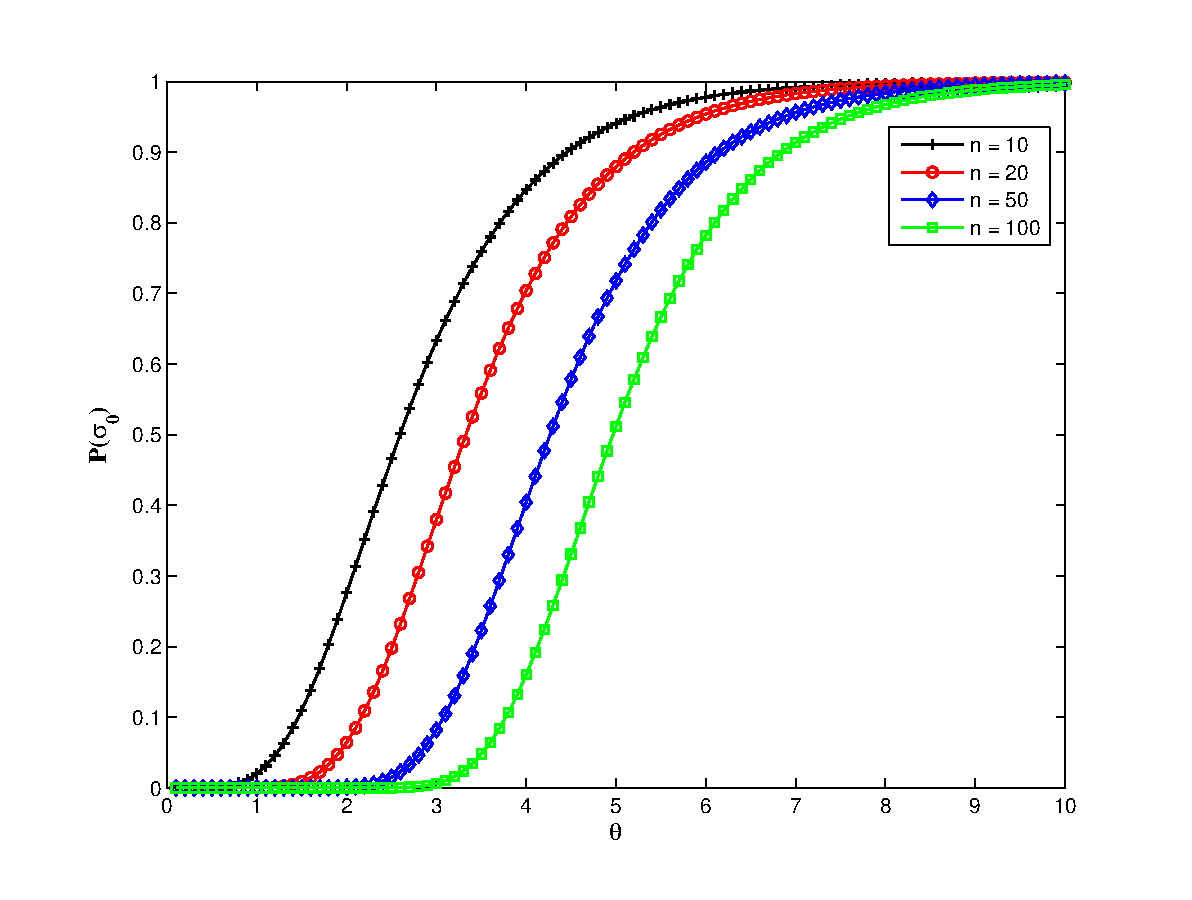
\epsfig{file=images/ProbabilityPlot4,height=7cm}
\caption{Probability assigned to $\sigma_0$ for different $\theta$ and $n$ values.}
\label{F:ProbabilityConsensuRanking}
\end{figure}

Based on these results, we completed a second set of experiments executing the Mallows EDA on some FSP instances. The $\theta$ parameter was fixed using a range of promising values extracted from the previous experiment. Particularly, we decided to use 8 values in the range [0,2]. These values are \{0.00001, 0.0001, 0.001, 0.01, 0.1, 0.5, 1, 2\}. The rest of the parameters typically used in EDAs are presented in Table~\ref{T:parameters}. Regarding the FSP instances, the first instance of each set \textit{tai20$\times$5, tai20$\times$10, tai50$\times$10}, \textit{tai100$\times$10} and \textit{tai100$\times$20}\footnote{\'{E}ric Taillard's web page. http://mistic.heig-vd.ch/taillard/problemes.dir/\\ordonnancement.dir/ordonnancement.html} was selected. Each experiment was run 10 times. Table~\ref{T:ThetaErrorRate} shows the error rate of these executions. This error rate is calculated as the normalized difference between the best value obtained by the algorithm and the best known solution.

\begin{table}
\centering
\scriptsize
\renewcommand{\arraystretch}{1.2}
\caption{Execution parameters of the algorithms. Being $n$ the problem size.}
\begin{tabular}{p{3.2cm}|p{5.5cm}}
Parameter & Value\\\hline
Population size & $10n$\\
Selection size & $10n/2$\\
Offspring size & $10n-1$\\
Selection type & Ranking selection method\\
Elitism selection method & The best individual of the previous generation is guaranteed to survive\\
Stopping criteria & $100n$ maximum generations or $10n$ maximum generations without improvement\\
\end{tabular}
\label{T:parameters}
\end{table}

\begin{table}[htbp]
\scriptsize
\centering
\caption{Average error rate of the Mallows EDA with different constant $\theta$s.}
\begin{tabular}{p{1.2cm}|x{1.5cm}|x{1.5cm}|x{1.5cm}|x{1.5cm}|x{1.5cm}}
\multicolumn{1}{c|}{$\theta$}& 20$\times5$ & 20$\times10$ & 50$\times10$ & 100$\times10$ & 100$\times20$
\tabularnewline\hline
0.00001 &0.0296 & 0.0930 & 0.1359 & 0.0941 & 0.1772\tabularnewline
0.0001 &0.0316 & 0.0887 & 0.1342 & 0.0917 & 0.1748\tabularnewline
0.001 &0.0295 & 0.0982 & 0.1369 & 0.0910 & 0.1765\tabularnewline
0.01 &0.0297 & 0.0954 & 0.1275 & 0.0776 & 0.1629\tabularnewline
0.1 &0.0152 & 0.0694 & 0.0847 & \textbf{0.0353} & \textbf{0.1142}\tabularnewline
0.5 &\textbf{0.0081} & 0.0347 & \textbf{0.0780}& 0.0408 & 0.1236\tabularnewline
1 &0.0125 & \textbf{0.0333} & 0.0936 & 0.0610 & 0.1444\tabularnewline
2 &0.0182 & 0.0601 & 0.1192 & 0.0781 & 0.1649\tabularnewline
\end{tabular}
\label{T:ThetaErrorRate}
\end{table}

The results shown in~\ref{T:ThetaErrorRate} indicate that the lowest or highest values of $\theta$ (in the [0,2] interval) provide the worst results, and as $\theta$ moves inside the interval the performance increases. Particularly, the best results are obtained for 0.1, 0.5 and 1 values.

\subsection{Testing the Mallows EDA on FSP}

Finally, we decided to run some preliminary tests for the Mallows EDA algorithm on the previously introduced set of FSP instances (taking in this case the first six instances from each file).
Taking into account the results extracted from the analysis of $\theta$, we decided to fix its initial value to 0.001, and to set the upper bound to 1. The parameters described in Table~\ref{T:parameters} were used for the EDAs. In particular, for NHBSA and EHBSA algorithms, $B_{ratio}$ was set to 0.0002 as suggested by the author in~\cite{Tsutsui06nodehistogram}.

For each algorithm and problem instance, 10 runs have been completed. In order to analyze the effect of the population size on the Mallows model, in addition to $10n$ we have also tested $n$, $5n$ and $20n$ sizes.

Table~\ref{T:ExperimentsPercent} shows the average error and standard deviation of the Mallows EDA and Tsutsui's approaches regarding the best known solutions. Note that each entry in the table is the average of 60 values (6 instances $\times$ 10 runs). Looking at these results, it can be seen that Tsutsui's approaches yield better results for small instances. However, as the size of the problem grows, both approaches obtain similar results for $50\times20$ instances, and the Mallows EDA shows a better performance for the biggest instances $100\times10$ and $100\times20$. The results obtained show that the Mallows EDA is better for almost all population sizes. These results stress the potential of this Mallows EDA approach for permutation-based problems.

\begin{table}
\centering
\scriptsize
\caption{Average error and standard deviation for each type of problem. Results in bold indicate the best average result found.}
\begin{tabular}{lc|x{1.5cm}|x{1.5cm}|x{1.5cm}|x{1.5cm}|x{1.5cm}|x{1.5cm}}
\multicolumn{2}{c|}{\multirow{2}{*}{EDA}} & \multicolumn{4}{c|}{Mallows}& \multicolumn{1}{c|}{EHBSA} & \multicolumn{1}{c}{NHBSA}\\
& & \scriptsize{\textit{n}} & \scriptsize{\textit{5n}} & \scriptsize{\textit{10n}} & \scriptsize{\textit{20n}} & \scriptsize{\textit{10n}} & \scriptsize{\textit{10n}}\tabularnewline\hline

\multirow{2}{*}{20$\times$5} & \scriptsize{\textit{avg.}} & 0.0137  & 0.0102 & 0.0102 & 0.0096 &\textbf{0.0039} &0.0066 \tabularnewline
& \scriptsize{\textit{dev.}} & 0.0042 & 0.0037 & 0.0035 & 0.0039  &0.0034 &0.0032 \tabularnewline\hline

\multirow{2}{*}{20$\times$10} & \scriptsize{\textit{avg.}} & 0.0357  & 0.0258 & 0.0250 &  0.0232 &\textbf{0.0065} &0.0076 \tabularnewline
& \scriptsize{\textit{dev.}} & 0.0054  & 0.0033 & 0.0037 & 0.0030 &0.0023 &0.0016 \tabularnewline\hline

\multirow{2}{*}{50$\times$10} & \scriptsize{\textit{avg.}} & 0.0392  & 0.0345 & 0.0342 & 0.0349  &\textbf{0.0323} &0.033	\tabularnewline
& \scriptsize{\textit{dev.}} & 0.0067  & 0.0071 & 0.0059 & 0.0062 &0.0066 &0.0069 \tabularnewline\hline

\multirow{2}{*}{100$\times$10} & \scriptsize{\textit{avg.}} & 0.0093 & \textbf{0.0078} & 0.0083 & 0.0089 &0.0199 &0.0157 \tabularnewline
& \scriptsize{\textit{dev.}} & 0.0040 & 0.0040 & 0.0045 & 0.0053 & 0.0047&0.0062 \tabularnewline\hline

\multirow{2}{*}{100$\times$20} & \scriptsize{\textit{avg.}} & \textbf{0.0583}  & 0.0610 & 0.0661 &  0.0587 &0.0676 &0.0631 \tabularnewline
& \scriptsize{\textit{dev.}} & 0.0116  & 0.0130 & 0.0132 &0.0121  &0.0050 &0.0071 \tabularnewline

\end{tabular}
\label{T:ExperimentsPercent}
\end{table}

\section{Conclusions and Future Work}

In this paper a specific EDA for dealing with permutation-based problems was presented.  We introduced a novel EDA, that unlike previously designed permutation based EDAs, is intended for codifying probabilities over permutations by means of the Mallows model. In order to analyze the behavior of this new proposal, several experiments have been conducted. Firstly, the $\theta$ parameter has been analyzed, in an attempt to discover its influence in the exploration-exploitation trade-off. Secondly, the Mallows EDA has been executed over several FSP instances using the information extracted from $\theta$ values in the initial experiments. Finally, for comparison purposes, two state-of-the-art EDAs have been executed: EHBSA and NHBSA. From these preliminary results, it can be concluded that the Mallows EDA approach presents an interesting behavior, obtaining better results than Tsutsui's algorithms as the size of the problem increases.

As future work, there are several points that deserve a deeper analysis. On the one hand, it would be interesting to extend the analysis of $\theta$ in order to obtain a better understanding of its influence: initial value, upper bound, etc. On the other hand, with the aim of ratifying these initial results it would be interesting to test this Mallows EDA on a wider set of problems, such as the Traveling Salesman Problem, the Quadratic Assignment Problem or the Linear Ordering Problem.

\section*{Acknowledgments} 
Thank you every one!
\bibliographystyle{abbrv}
\bibliography{./bibliography.bib}
\end{document}
